\documentclass[runningheads]{llncs}

\usepackage[T1]{fontenc}
\usepackage{cite}
\usepackage{graphicx}
\usepackage{graphicx} % Required for inserting images
\usepackage{hyperref}
\usepackage{float}
\usepackage{xcolor}
\usepackage{amsmath} % begin{aligned}
\usepackage{amsfonts} % \mathbb{}
\usepackage{todonotes} % \todo and \todo[inline]
\usepackage{tabularx}

\newcommand{\xor}{\oplus}
\newcommand{\toref}[1]{\todo[color=yellow]{#1}}
\newcommand{\tothink}[1]{\todo[color=pink]{#1}}
\newcommand{\bigO}[1]{$\mathcal{O}(#1)$}

\begin{document}
	
	\title{Generating trusted sphinx packets}
	
	\author{Anonymous}
	\authorrunning{Anonymous}
	\institute{}
	
	\maketitle 
	
	\begin{abstract}
		We propose a decentralized scheme that prevent mixnets users from sending traffic that does not match the service provider of an anonymous credential. Our scheme is of direct use in the Nym network where users construct an anonymous credential given they receive a certificate of them paying for that service provider. Our scheme prevent users from cheating by using a credential for a free service and send traffic for a paid service. Our solution works even if the majority of the third parties collude. Finally we evaluate the performance of our solution.
		\keywords{mixnet \and sphinx \and malicious users}
	\end{abstract}


\section{Introduction}

Mix network, or mixnet, is an overlay network of servers (called mix nodes) that prevent an adversary from correlating senders with receivers~\cite{chaum-mix,cypherpunk-remailer,piotrowska2017loopix,nym-network-whitepaper,danezis2003mixminion, van2015vuvuzela,mixmaster-spec,chaum2016cmix}. They achieve this by adding delays to messages inside the different mixnodes in order to mitigate timing analysis attacks. Additionally, unlike Tor~\cite{onion-routing96} where all packets sent by a user follow the same path for the entire session (called circuit-based), in mixnets routing is typically packet-based (meaning that each packet follows a different path). These two techniques ensure that mixnets are resilient against a strong adversary who observes the entire input and outputs of the network typically called a Global Passive Adversary (GPA).
During the last few decades several systems have been proposed in the literature and few of them have been implemented. Open research problems such as parameterization, authentication and fake dummies have halted the usage on a large scale.
%
\todo{what are \enquote{fake dummies} do we still say \enquote{dummies} :-s}
%
Recently, Nym Technologies a mixnet-based company is being commercialized
and proposing a mixnet network for services to be integrated with their
network for a fee. Their network is based on
Loopix~\cite{piotrowska2017loopix}. Users of these services are then
allowed to use the Nym mixnet by using Nym credentials (based on the
Coconut credential~\cite{coconut}) that they can construct after getting a
certificate of paying for a specific service to use the Nym network.
However, nothing prevents users from cheating who might exploit a valid Nym
%
\todo{Can we quantify the impact somehow? Show that this is a real problem?}
%
credential for another service they did not pay for. This is a particular
difficult problem in anonymous communication networks where the mixnodes do
not know the traffic type or the final service a user is communicating with
by doing layered encryption where the final IP address is only know by the
last node in the path using a packer format such as Sphinx~\cite{sphinx}. 

In this paper we present a scheme that creates the Sphinx header in a
decentralized way based on trusted third parties while ensuring that these
parties learn nothing about the destination or the path.
%
\todo{This sentence needs something more about the preventing cheating and
reduction of overheads.}
\todo{From our call 2025-06-10: \enquote{While it's computationally more complex, our schema does not allow the mixnet to ge saturated by an attacker.}}
\todo{Would there be a risk of unauthenticated attacker-controlled traffic
somehow breaking anonymity?}
%
Our work makes the
following contributions:
%
\begin{itemize}
%
  \item{\ldots}
%
  \item{\ldots}
%
  \item{We assess the impact on availability and economic viability
adversaries can have in Sphinx and our solution and conclude that\ldots}
%
\end{itemize}
%
\todo{Something on prototype and availability of artifacts!}
\todo{For CBT: highlight relevance of the contribution to Lightning and Nym
in intro and contributions.}

We highlight related work and motivation in Section~\ref{sec:related}, then we specify and justify our system model in Section~\ref{sec:sys_model}, where we also describe the considered threat model. We then present our scheme that decentralize the creation of the Sphinx headers in Section~\ref{sec:scheme} and the evaluation of our proposed solution in Section~\ref{sec:eval}. Finally we conclude and discuss future work in Section~\ref{sec:conclusion}

\section{Motivation and Related Work}
\label{sec:related}

Since Chaum’s seminal work on untraceable email in 1981~\cite{chaum-mix}, there has been a great amount of research related to mixnets' design~\cite{piotrowska2017loopix, van2015vuvuzela, kwon2020xrd, lazar2018karaoke, cottrell1995mixmaster, alexopoulos2017MCMIX, chaum2016cmix, chaum-mix, danezis2003mixminion}. However most systems that have been deployed and used come with their own system on top of the network meaning that only one type of traffic type is allowed. As beautifully stated by Dingledine et al. in~\cite{dingledine2006anonymity}, "Anonymity Loves Company" meaning that the more messages there are in the network the more privacy the network provide. This is also shared by Ben Guirat et al. in~\cite{benguirat2023blending} where the authors show that blending different traffic types on top of a mixnet provide better anonymity, meaning let's imagine an instant messaging system where users do not tolerate latency of more than few seconds and an email app where users tolerate latency of up to 1 minute. The authors show that blending these two types of traffic do actually increase the privacy for both traffic. This only applicable in networks such as Tor or the Nym network that they offer the network for different applications to be integrated on top of the network rather than dictating which application to use the mixnet.
However, certain open research problems remain open. For example how can we ensure that certain traffic are not allowed (for whatever reason and we will specify the exact reason for our work) without compromising ?
Tor solves the problem with having exit policy that simply drop traffic at the last node. However Tor routing is circuit-based meaning that all traffic from a specific user session follow one path and hence packets are encrypted using symmetric cryptography which is cheap, so even if traffic is dropped that is not a problem.

However, and beyond Tor, mixnets can impose substantial computational
overheads due to packet based routing where every packet takes a different
path and hence layered public-key cryptography is used. This implies that
that, if packets are dropped at the last node of the mix, which is
traditionally the only place where service contracts can be validated,
computational resources required by the mix to propagate a packet to its
final node are wasted. Additionally, and unlike Tor where relaying traffic
happens on a volunteering base, nodes in mixnets such as Nym are
economically incentivized through payment per relayed bandwidth. Thus,
dropping packets at an the exit node impacts the economic viability of the
mixnet service.

\begin{questions}
%
        \item \ldots
%
\end{questions}
%
\todo{Some concrete research questions that we can derive here and answer?}





\section{System and Threat Model}~\label{sec:sys_model}

We observed that adversarial interactions on mixnets can increase the use of
computational resources and network resources, thus reducing the
availability and negatively affecting economic viability of mixnet
services. Our work seeks to mitigate these challenges. Below we describe
the system model and the adversary we consider, and derive privacy and
security requirements for our solution.

\subsection{System Model}

\todo{Aurelien: I think we could try to be more concise on this subsection
because it feels quite heavy (especially the second half speaking of
coconut and blockchain).  But for the moment, this part is a bit tricky
since we haven't really focus on credentials...}
%
\todo{Iness: add a simple graph here of a mixnet; purpose: illustrate
system model, benign interactions, adversarial interactions.}
%
We abstract the Nym mixnet to the components that are relevant for our
work. We consider a mixnet, where each user have a gateway that shows a
credential and if accepted their traffic is allowed.  To prevent
correlation, mixnet relies on fixed-size packet format such as Sphinx
packet, making it difficult for external
observers to link incoming and outgoing messages at any given node.  The
Nym credential is constructed by the user and issued by a third
decentralized party after obtaining a certificate that proves payment.  For
example let's say Signal is integrated with Nym, and Signal users who want
their traffic to be anonymous instead of sending traffic directly to the
Signal server, traffic will be first routed through the mixnet such that an
adversary who observes the signal server and/or the device of the user can
not correlate the sender with signal server and eventually the final
recipient. Signal (service provider) can add an option for user who want to
pay and issue a certified attribute to those users. Users then encode this
attributes into a credential and sends it to validators. If the proof is
valid, validators return partial signatures. Once the user collects a
threshold number of these signatures, they aggregate them to form a valid
credential and re-randomize it to ensure unlinkability from previous
interactions. The user can then present this credential to a verifier to
prove their right to access a service to show that the credential meets all
necessary payment and authentication conditions. To prevent
double-spending, the verifier checks that the credential has not already
been used by consulting the blockchain and then commits the credential's
serial number to the blockchain upon acceptance.  For example, a user can
obtain an certification from the Signal service provider, construct a valid
credential and then use it to route traffic to another service provider
they didn't pay for or simply not allowed (an illegal website).  Such
misuse would be detected only at the final node of the mixnet preventing
the user from accessing another application.  However, prior mixnodes would
have already wasted computational resources processing an invalid packet.
This vulnerability enables Denial of Service (DoS) attack by exhausting
mixnodes computational power with illegitimate packets.

Additionally, each encryption layer includes an integrity tag, which prevents tampering and improves the network’s resistance against malicious mixnodes and active adversaries.

\subsection{Threat Model} 

We consider different types of adversaries:
\todo{Aurelien: I feel like the bullet points are mixing a bit threat model (GPA, malicious user and honest-but-curious TTP) with desired properties (collusion resistant, integrity, unlinkability, ...)}
\begin{itemize}
	\item A GPA: an adversary who is able to observe all the inputs and outputs of the network. This adversary should not be able to correlate an input with an output based on the packet's appearance. This is achieved by the bitwise unlinkability of the sphinx packets.
	\item When constructing the headers: By using a Trusted Third Party that constructs the headers we need to make sure that even if the majority of the entities collude, no one should know the final destination of the user.
	\item An adversary who captures the headers is not able to change headers without intervening with the integrity check and hence mixes are able to know that the integrity check has been tampered with.
	\item Malicious users: Users can not cheat and create their own headers and putting the final destination different from the one they have the credential for.
\end{itemize}

\subsection{Security \& Privacy Objectives}
\label{sec:sp-objectives}

\begin{objectives}
%
        \item Cheating users: Users' traffic is only allowed to be routed
if the traffic belongs to the same service provider from the credential
%
        \item even if the majority of headers issuers are colluding, they
do not know which service provider the user is communicating with.
%
        \item the Spinx headers can not be altered.
%
        \item Verifiers can verify that the headers has not been altered
without revealing the service provider.
%
        \item Unlinkability between  sphinx packets, the original sphinx
packet that is constructed in a centralized way provide the
\textit{unlinkability} property, meaning that an adversary can not know
that two packets are connected to the same user. Our scheme that
decentralize the headers creation aim at providing this same property.
%
\end{objectives}
\todo{Some objectives may need a bit of explanation re. why they matter,
for others I'm not sure how they can be evaluated.}



\section{Sphinx}
\todo{Iness: This entire subsection explains the original sphinx packet format, I think it's too much and can be reduced to 20\%. The rest can be either be deleted or used on how you construct the decentralized scheme}
Sphinx packets consist of a header and an encrypted payload. 
The header itself contains a \textit{cryptographic element $\alpha$} (e.g. $g^x$ or an elliptic curve point), \textit{encrypted routing information $\beta$}, and an \textit{integrity tag $\gamma$}, as illustrated in Figure \ref{fig:sphinx_structure}.

\begin{figure}[h]
    \centering
    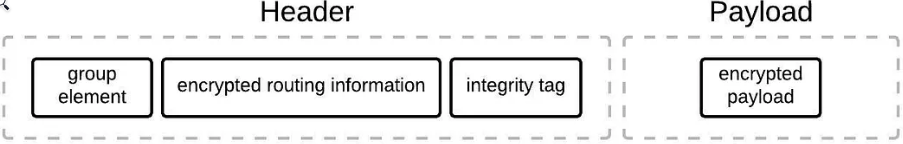
\includegraphics[width=0.9\linewidth]{Images/sphinx_structure.png}
    \caption{Structure of sphinx packet. \href{https://blog.nymtech.net/sphinx-tl-dr-the-data-packet-that-can-anonymize-bitcoin-and-the-internet-18d152c6e4dc}{[source]}}
    \label{fig:sphinx_structure}
\end{figure}

The \textit{encrypted routing information ($\beta$)} is constructed in layers, applied in reverse order along the path.
First, the final destination is encrypted, and an integrity tag ($\gamma_i$) is computed. 
The IP address of the last mixnode ($n_i$) is then prepended.
As shown by Figure \ref{fig:sphinx_header}, this process repeats iteratively: each new header is encrypted, an integrity tag ($\gamma_{i-1}$) is computed, and the IP address of the preceding mixnode ($n_{i-1}$) is prepended.
This layered encryption ensures that each mixnode can only decrypt its own layer, revealing the next forwarding address while preserving end-to-end confidentiality and protecting against tampering.

\begin{figure}[h]
    \centering
    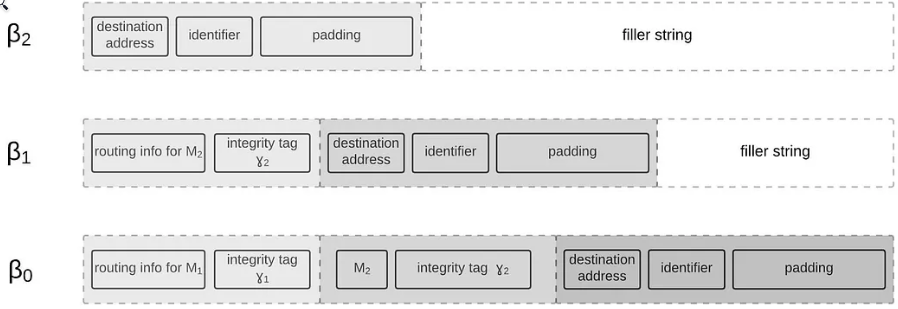
\includegraphics[width=\linewidth]{Images/sphinx_header.png}
    \caption{Sphinx encrypted routing information encapsulation. \href{https://blog.nymtech.net/sphinx-tl-dr-the-data-packet-that-can-anonymize-bitcoin-and-the-internet-18d152c6e4dc}{[source]}}
    \label{fig:sphinx_header}
\end{figure}

To encrypt the routing information, the Nym client\todo{previously "user" but JT prefers "Nym client"} first chooses a nonce $x$ and compute $\alpha = g^x$ as the \textit{cryptographic element} of the header.
Since each mixnode $i$ has a private key $x_i$ and a public key $y_i = g^{x_i}$, the user can create a shared secret $s_i$ with mixnode $i$ as followed: $s_i = y_i^x = (g^{x_i})^x$. 
Then the mixnode $i$ receiving the packet will get $\alpha$ allowing him to compute the shared secret as followed: $s_i = \alpha^{x_i} = (g^x)^{x_i}$.

Instead of sending a unique \textit{cryptographic element $\alpha$} at each node in the path, the sphinx format uses a single \textit{cryptographic element $\alpha$}, which is progressively modified at each node. 
Each mixnode updates the cryptographic element using its shared secret as follows:  
$$\alpha_{i+1} = \alpha_i^{\text{hash}(\alpha_i, s_i)}$$
Thus, the user iteratively computes the shared secrets in the path's order as: 
$$
\begin{aligned}
    \alpha_0 &= g^{x}, & s_0 &= y_{n_0}^{x}, & b_0 &= \text{hash}(\alpha_0, s_0) \\
    \alpha_1 &= g^{x b_0}, & s_1 &= y_{n_1}^{x b_0}, & b_1 &= \text{hash}(\alpha_1, s_1) \\
    &\vdots & &\vdots & &\vdots \\
    \alpha_i &= g^{x b_0 \cdots b_{i-1}}, & s_i &= y_{n_i}^{x b_0 \cdots b_{i-1}}, & b_i &= \text{hash}(\alpha_i, s_i)
\end{aligned}
$$
This formulation ensures that each mixnode can independently derive the necessary cryptographic elements without requiring the full path’s information, preserving privacy and unlinkability.  
\newline

The \textit{encrypted routing information ($\beta$)} is computed, as illustrated in Figure\todo{$\sim$\textbackslash ref\{\}} \ref{fig:sphinx_header}, by processing the path in reverse order. 
This involves XORing the routing information ($\beta_{i-1}$) from the previous layer (with the node's address and integrity tag) with a value derived from the shared secret $s_i$. 
Then prepending this new encrypted routing information ($\beta_i$) with an integrity tag ($\gamma_i$) and the previous mixnode address (remember we build it in reverse order).
We repeat the same process for each layer (i.e. each mixnode in the path).

\begin{figure}[H]
    \centering
    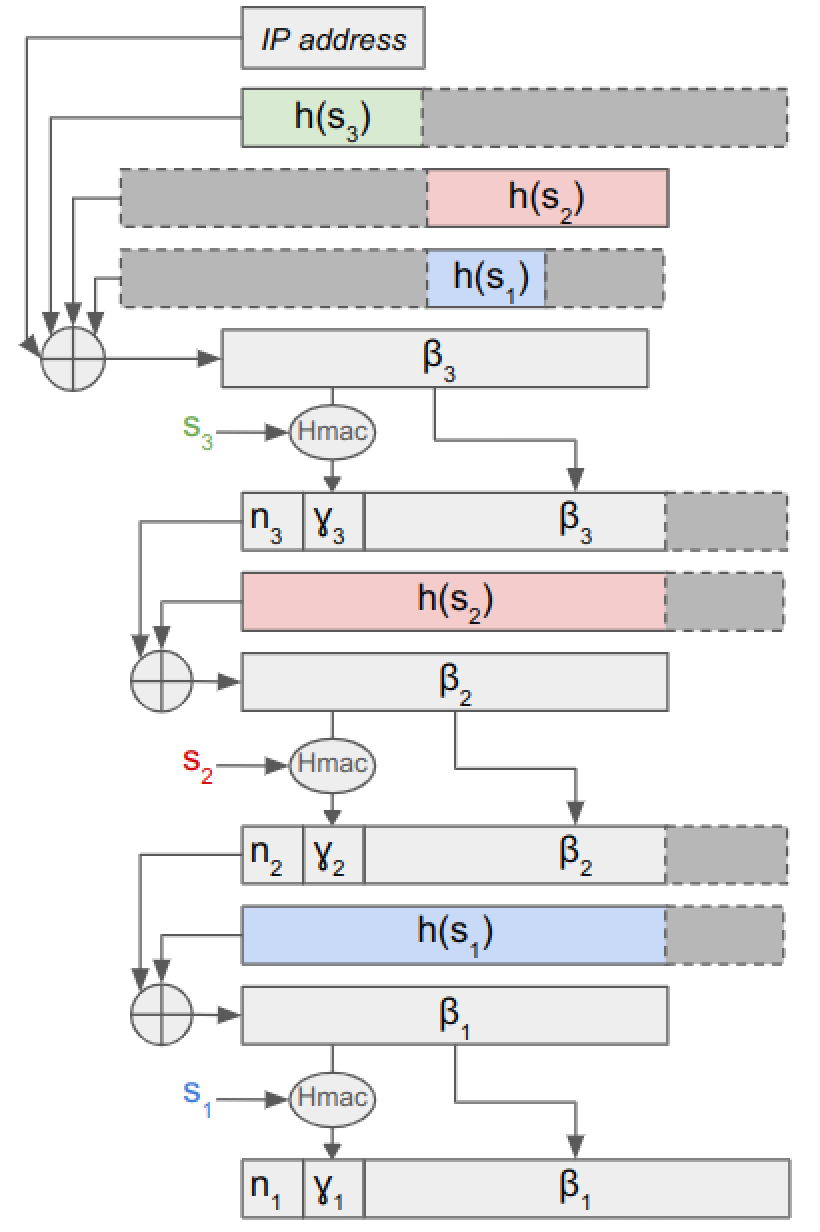
\includegraphics[width=0.5\linewidth]{Images/header_cipher.png}
    \caption{Construction of the Sphinx header (modified from \cite{sphinx}) [TO FIX: $h(s_1)$ at first XOR]}
    \label{fig:header_cipher}
\end{figure}
\todo[inline]{JT: Explain what the modifications are}
\todo[inline]{JT: Might help to put some (1) (2) (3) labels into the figure and refer to these labels in the text.}

% first round
The first round of XOR operations differs from the others because it requires combining parts of all shared secrets. 
Specifically, the destination address is XORed with the last node’s shared secret, truncated to match the address size.
Next, the result is concatenated with the XORed values of the ending parts of the shared secrets from the other nodes in the path. 
This ensures that when the entire header is XORed with the full shared secret, these appended values cancel out, allowing the header to be processed in reverse order by the mixnodes.
This design choice guarantees fixed-size headers, enabling fixed-size packets which is a crucial property in mixnets for maintaining unlinkability.

\todo[inline]{JT: Now maybe follow up with an example of the attack from the introduction?
We should also compare computational overheads from attack vs. the new protocol design.}

%%%%%%%%%%%%%%%%%%%%%%%%%%%%%%%%%%%%%%%%%%%%%%%%%%%%%%%%%%%%%%%%%%%%%%%%%%%%%%%%%%%%%%%%%%%%%%%%%%%%%%%%
%%%%%%%%%%%%%%%%%%%%%%%%%%%%%%%%%%%%%%%%% Our solution %%%%%%%%%%%%%%%%%%%%%%%%%%%%%%%%%%%%%%%%%%%%%%%%%
%%%%%%%%%%%%%%%%%%%%%%%%%%%%%%%%%%%%%%%%%%%%%%%%%%%%%%%%%%%%%%%%%%%%%%%%%%%%%%%%%%%%%%%%%%%%%%%%%%%%%%%%

\newpage
\section{Our Solution - Multi-Party Computation (MPC)}\label{sec:scheme}
\todo[inline, color=blue!30]
{
    [NOTE] - To do or improve
        \newline- Carefully select variable's notation, e.g. h, h(), H() and hash();
        \newline\hspace*{1cm} - Don't like $\alpha$ notation since it should be capital letter (point)
        \newline\hspace*{1cm} - Should use $\Gamma$ instead of $\gamma$ notation (point)
        \newline\hspace*{1cm} - And what about $\beta$, $b$, $x$, ...
        \newline- Do or improve schemas;
        \newline- Clarify that we work with a path of length 3 (could be generalized)
}

Our approach to ensure trust in the Sphinx header is to prevent user manipulation by decentralizing the header construction to Trusted Third Parties (TTP) through the use of Multi-Party Computaftion (MPC).
\newline

We consider TTPs as \textit{honest-but-curious}.
This means that they follow the protocol correctly but may attempt to infer additional information from the data they process.
Our design ensures that TTPs cannot infer any information about the shared secrets $ s_i $ or the involved mixnodes, even when TTPs collude (except one).
\todo{JT: In the Nym ecosystem, who are the TTPs, who operates them, what exactly are they trusted for?}

\subsection{Development Path / Thinking path}

Before introducing our decentralized schema, we briefly outline the key decisions that shaped our implementation.
\newline

\noindent We considered three main approaches to decentralize the Sphinx header computation:
\begin{enumerate}
    \item \textbf{Distributed:} Each TTP computes a distinct layer (sequential approach);
    \item \textbf{Partially decentralized:} All TTPs compute a layer based on partial information, aggregate their results to compute the integrity hash, redistribute the outcome, and repeat the process with the next layer;
    \item \textbf{Fully decentralized:} All TTPs compute the full Sphinx header using partial information, and their results are aggregated at the end.
\end{enumerate}

The first approach compromises privacy, as each TTP learns two consecutive nodes in the path and one of the associated shared secrets, raising serious security concerns.
The second approach increases communication overhead and allows the aggregating TTP to observe the intermediate Sphinx header at specific stages, which could enable packet tracking if the aggregator colludes.
Finally, the third approach was selected for its stronger privacy guarantees, despite its added complexity.
\newline

% hash -> Homomorphic encryption
The main challenge in the fully decentralized setting lies in the integrity tag which relies on a hash function. 
Although a homomorphic hash would be ideal to support decentralized hash, such construction remains poorly studied and potentially weaken its security due to the homomorphic additive or multiplicative nature (easier for collisions).
As a practical workaround, we substitute the hash with a one-way homomorphic encryption scheme (only encryption, not decryption). 
More specifically, a homomorphic encryption with mutually commutative operators (like RSA and ElGamal but not Paillier) due to the nested structure of the integrity tag, which contains previous tags.
\todo[color=blue!30]{Should I develop why ?}

%%% Size -> ECC -> 1 Point per element -> cut in chunks
To improve efficiency, we switch from RSA-like primitives to elliptic curve cryptography (ECC), which offers more compact representations while keeping these homomorphic properties.
By abstracting away encryption layers, the final header is structured as follows: 
\[
[\text{node 1, integrity 1, node 2, integrity 2, node 3, integrity 3, destination}]
\]
\todo[color=blue!30]{adding a figure to illustrate ?}
Since deriving all these information from just one or two EC points seems impractical, we represent each piece of information by an EC point.
To achieve this, we split the encoded string into chunks as represented by Figure \ref{fig:chunked_schema}, each corresponding to a single EC point.

\begin{figure}[H]
    \centering
    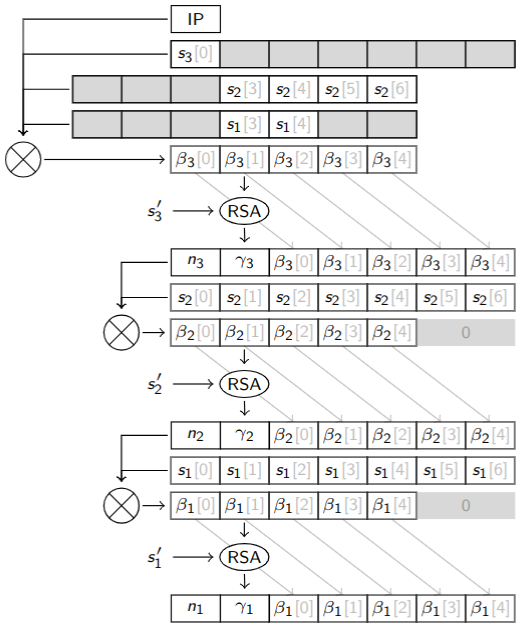
\includegraphics[width=0.6\linewidth]{Images/chunked_structure.png}
    \caption{Chunked representation of the schema}
    \label{fig:chunked_schema}
\end{figure}

\todo[color=blue!20]{Nice guidelines ref: RFC9380 (Hashing to Elliptic Curves)}
One remaining challenge when encoding information into elliptic curve (EC) points is the decoding process.  
Some type of data such as IP addresses (destination or mixnodes) requires both an encoding method that maps an integer to a point and a corresponding decoding method that retrieves the integer from the point.
In this article, we refer to these two processes respectively as \textit{integer-to-point} noted $H()$, and \textit{point-to-integer} noted $h()$.
\newline

A classical approach to achieve such a mapping involves the x-coordinate of the point.
The point-to-integer function simply returns the x-coordinate of the point.
The integer-to-point function computes the y-coordinate where x is the integer.
However, a randomly chosen x-coordinate will lie on the curve only about 50\% of the time.  
A simple workaround is to increment the x-coordinate until a valid point is found.  
Yet, this technique introduces a problem in our context since the x-coordinates correspond to IP addresses. 
Nearby IPs could map to the same point, potentially leading to collisions that compromise correctness of the mixnet.
This risk could be mitigated by padding the IP with a random fixed-length binary string.
\newline

From our knowledge, a second alternative exists: the Elligator 2 algorithm.  
Elligator provides a method to map any integer to a pseudo-random point on a Montgomery curve in a uniform and reversible way.  
More precisely, the reverse mapping (point-to-integer) requires that the point satisfies specific mathematical conditions, which occur with roughly 50\% probability for a random point.  
Again, a simple workaround is to increment the point by adding the curve's generator until the point fulfills these conditions.

Note that all points derived from integers using Elligator are guaranteed to be reversible.  
Thus, a point representing an IP address (which originally comes from an integers) can always be correctly decoded.  
Only random points used as shared secrets may require few extra point additions to meet these conditions which represents a negligible computational overhead.
\newline

To summarize, we need a mapping that is as bijective as possible but we face a trade-off between two imperfect scenarios:
\begin{itemize}
    \item A complete and easily reversible point-to-integer mapping (i.e. using x-coordinates), but only partial coverage for integer-to-point.
    \item A complete integer-to-point mapping (i.e. using Elligator), but only partial coverage for point-to-integer.
\end{itemize}

Elligator seems a better solution since it guarantees stronger security/privacy by providing a more uniformly distributed output.
Moreover the complete integer-to-point is more important (to prevent IP collision) and we can deal with partial point-to-integer mapping in our use case.

\newpage
\todo[inline, color=blue!30]{
    It feels a bit heavy with too much details and remarks. 
    The whole previous page could be reduced to this shorter alternative.
    Which one is better ?
    \newline

    [Alternative shorter version]: \newline
    One remaining challenge lies in encoding and decoding information to and from elliptic curve points. 
    Specifically, we require a pseudo-random mapping between integers field and curve points group.
    
    Traditional methods achieve this by directly mapping integers to the x-coordinates of points on the curve. 
    However, this approach could leaks information by introducing bias since nearby integers result in nearby points.
    
    To address this, we adopt Elligator, which offers stronger privacy guarantees. 
    Unlike the traditional approach, Elligator produces a uniformly distributed output which is computationally indistinguishable from truly random curve points. 
    This uniformity is critical in our context, where preserving anonymity and avoiding linkability are core goals.
}

\subsection{Protocol description}

The overall decentralized scheme is illustrated in Figure~\ref{fig:overall_schema}.  
The client first computes a sequence of shared secrets and then splits these secrets, along with the IP addresses of the mixnodes in the path and the final destination, into $m$ shares.  
Each set of shares is sent to a different TTP, along with the necessary cryptographic element ($\alpha$).  
Each TTP independently computes a \textit{partial} Sphinx header using the received shares.  
The client then aggregates these partial headers to reconstruct the final header, ready for transmission through the mixnet.

\begin{figure}[H]
    \centering
    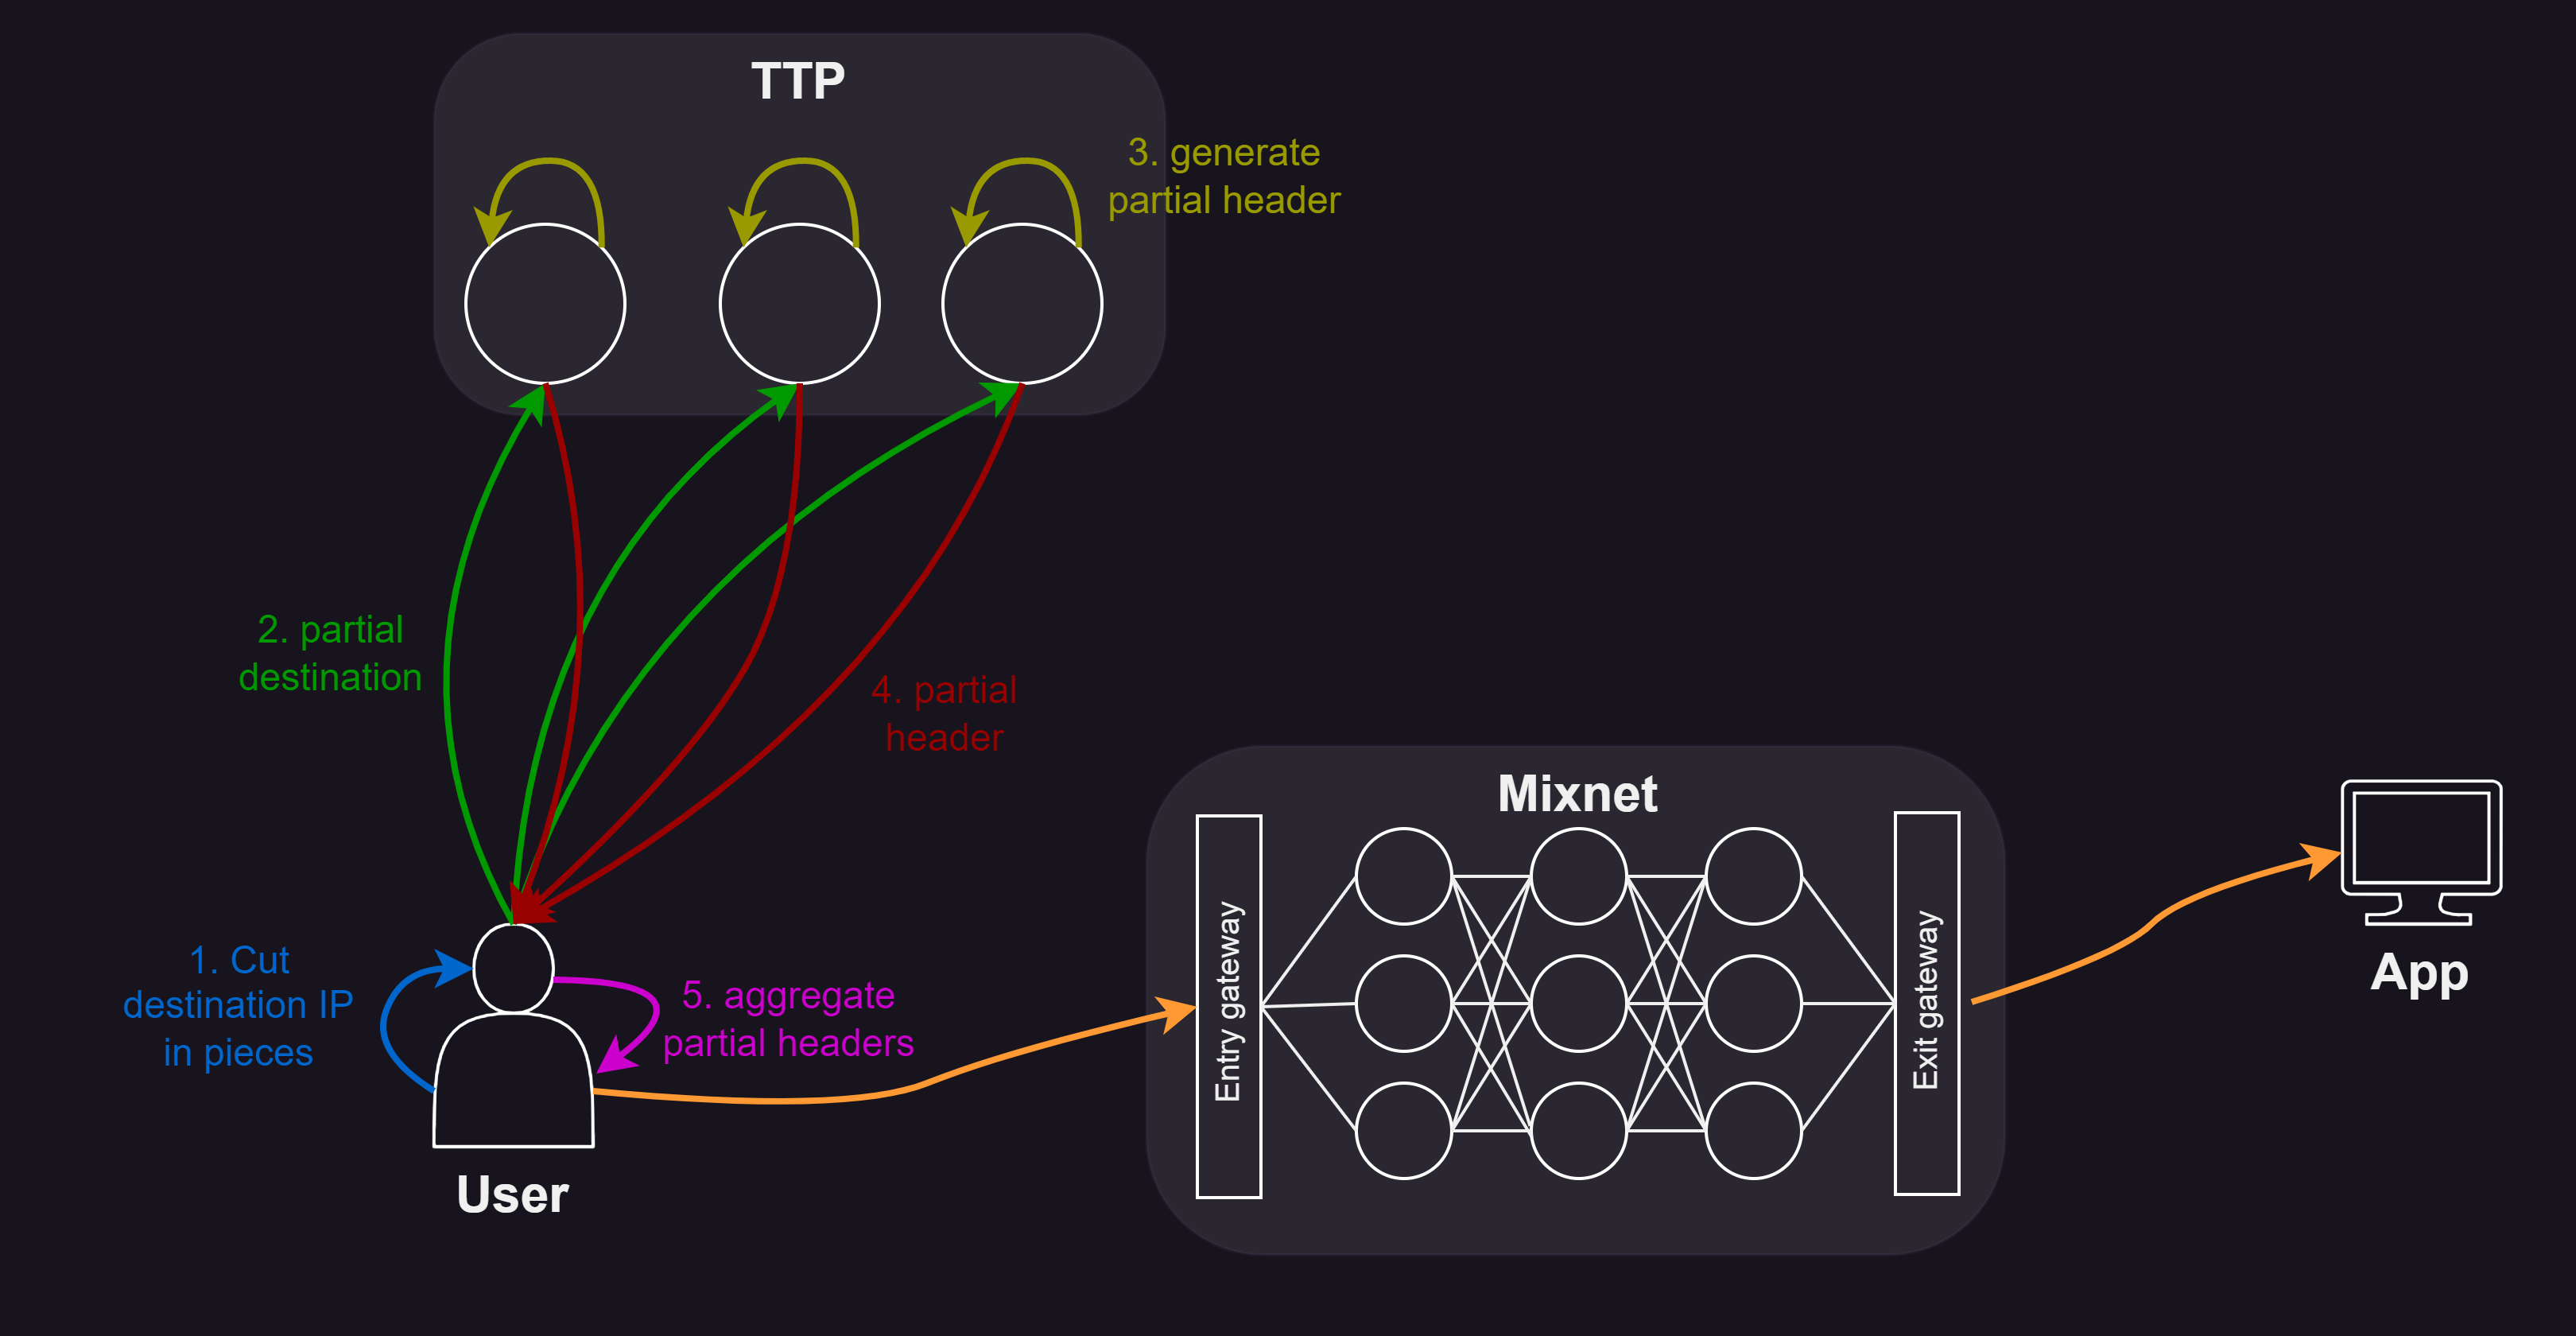
\includegraphics[width=1\linewidth]{Images/sphinx_ttp.png}
    \caption{Overview of the decentralized scheme}
    \label{fig:overall_schema}
\end{figure}

\noindent In summary, the protocol is divided into four main steps:
\begin{itemize}
    \item \textbf{Setup}: fixes random points as \textit{generators} (once but should be refreshed);
    \item \textbf{Client}: \textit{splits and shares} the necessary information to TTPs;
    \item \textbf{TTP}: \textit{encrypts} the routing information into a partial header;
    \item \textbf{Mixnode}: \textit{decrypts} and forwards the header.
\end{itemize}


\subsubsection{Setup}

In our protocol, routing information is divided into seven chunks (see Figure \ref{fig:chunked_schema}), each one encoded into an elliptic curve point. 
These points will later be encrypted by adding a masking point of the form $ P = s G $, where $ s $ is a shared secret and $ G $ is the base generator of the curve.
However, using the same masking point $ P $ for all the seven chunks compromises the \textit{unlinkability} property
(see security note in the TTP step \ref{note:security_why_indep_generators}).

To mitigate this, we use a set of seven \textit{independent} generators $ G_i $, one for each chunk. 
By \textit{independent}, we mean that the scalar relationship between any two generators is unknown. 
Therefore no one knows the scalars $ x_i \in \mathbb{Z}_N $ such that $ G_i = x_i G $.

In principle, this setup phase can be executed only once. 
However, to preserve unlinkability, the set of generators should be refreshed periodically. 
Every entity (clients, mixnodes, and TTPs) must run the setup phase to ensure they use the same set of generators.

To achieve synchronized and deterministic generator values across the system, we derive them from a common seed. 
This seed is computed as the hash of the current timestamp, truncated to the chosen refresh interval. 
To produce distinct seeds for each generator we rehash the seed, or simply increment it since Elligator already provides a uniform (i.e. pseudo-random) integers to points mapping.
\todo[color=blue!30]{In the current implementation, instead of incrementing the seed, we rehash it for each i. However, since Elligator produces uniformly distributed outputs, incrementing may be equally secure and more efficient.}

A subtlety with Elligator is that it can map integers to points outside of the base generator's subgroup.
Thus, an extra step is required to \textit{clear the cofactor} by multiplying the resulting point by the cofactor $ h $ (for Curve25519, $ h = 8 $).

\noindent The final formula for generating the $ i^{th} $ chunk’s generator is:
$$
G_i = h \cdot H(\text{hash}(\text{timestamp}) + i), \quad \text{for } i = 1, \dots, 7
$$


\subsubsection{Client}
% 1) Define a destination
% 2) Select a random path
% 3) Select a random salt $x$ (nonce) 
% 4) Generate a chain of shared secret for the path's mixnode
% 5) Transform IP addresses (path's mixnodes and destination) into Point with Elligator and the split those point into shares.
% 6) Split the shared secrets (int) into shares.
% 7) Send sets of shares (mixnodes IPs, destination IP, shared secrets) to different TTP.
% 8) TTP will compute from those shares a partial header and send it to the client. Afterwards, the client aggregate these partial headers.
  
To send a message to a specific destination, the client first randomly chooses a path through the mixnet and generates a nonce.
Using this nonce and the public keys of each mixnode along the path, the client derives a chain of shared secret integers $ (s_1, s_2, s_3) $ as follows:
\todo[inline,color=blue!30]
{
    Does it seems strange to transform the shared secret point into integer ?
    Should I explain why we need integer form ? 
    It might be a bit heavy and add too much details...
}
$$
\begin{aligned}
    \alpha_i    &= x_i \, G \\
    S_i         &= x_i \, \text{PK}_i \\
    s_i         &= h(S_i) \\
    b_i         &= \text{hash} ( {\alpha_i}_y \ \| \ {S_i}_y ) \\
    x_{i+1}     &= x_i \, b_i \quad (\text{mod}\ N)
\end{aligned}
$$
\todo[color=blue!30]{Order of equation lines ? and names of variables (espacially $x_i$ and $b_i$) ?}
where $ x_1 $ is the client's nonce, $ \text{PK}_i $ is the public key of the $ i^{th} $ mixnode in the path, 
$ N $ is the prime order of the elliptic curve group, $ \| $ is  the concatenation operator and subscript $ y $ refers to the $ y $-coordinate of the point.
The scalar $ b_i $ acts as a pseudo-randomizer to update the secret $ x_i $ for the next hop, 
ensuring that each cryptographic element $ \alpha_i $ remains unlinkable across mixnodes.

The IP addresses of the mixnodes and the destination are padded with random bits
then mapped to elliptic curve points using Elligator, allowing later recovery of these addresses.
\todo[color=red!40]{Test code: to verify if the padding is still necessary or optionnal and if limited (max size N)}
Both the resulting IP points and the shared secrets are split into shares and distributed to $ m $ different TTPs. 
\todo[inline, color=blue!30]{Should I mention how to split point (or integer) into $ m $ shares ? 
It is just taking $ m - 1 $ random points (or integers), sum them and compute the difference with the original point (or integer).}


Each TTP then independently computes a partial header from the received shares and returns it to the client. 
The client aggregates these partial headers by performing chunkwise point additions to reconstruct the complete encrypted header.
Finally, the client sends the header along with $ \alpha_1 $ to the first mixnode from the path. 
\todo[color=blue!30]{Do we need to remind that the user need to encrypt his message using these shared secrets (as in original article) or is uninteresting/obvious enough ?}

\subsubsection{TTP}
% 1) Receive partial destination, path's nodes and partial shared secret
% 2) First
% 3) For each layer
Each TTP receives from the client:
\begin{itemize}
    \item a share of the destination address (as an elliptic curve point),
    \item a share of each mixnode address in the path (as elliptic curve points),
    \item a share of each shared secrets (as integers).
\end{itemize}

The TTP constructs a partial encrypted header by layering routing information in reverse path order, starting from the last mixnode.

At each layer, two new chunks are introduced: the next mixnode’s address (as an EC point) and an integrity tag.  
To preserve a fixed-length header while allowing mixnodes to reverse the operation (as in the original design), four additional \emph{filler chunks} are appended.  
These filler chunks are carefully computed such that at each layer, after applying the corresponding masking points ($s_i \ G_j$), the last two chunks cancel out and become identity point (i.e. point at infinity).  
This mechanism allows these two chunks to be safely truncated at each layer, ensuring a consistent header size while preserving reversibility for mixnodes.

To initialize the header, the TTP encrypts the destination point using the shared secret of the last mixnode and append the required filler chunks. 
Let $ \Delta $ be the partial destination point, $ s_i $ the shared secret corresponding to the $ i^\text{th} $ mixnode in the path, and $ G_j $ the $ j^\text{th} $ chunk's generator. 
The chunks for the last layer (layer 3, assuming a 3-hop path) are computed as follows:

\[
\begin{aligned}
    {\beta_3}_1 &= \Delta       + s_3 \ G_1 \\
    {\beta_3}_2 &= - (s_2 \ G_4 + s_1 \ G_6) \\
    {\beta_3}_3 &= - (s_2 \ G_5 + s_1 \ G_7) \\
    {\beta_3}_4 &= - s_2 \ G_6 \\
    {\beta_3}_5 &= - s_2 \ G_7 \\
\end{aligned}
\]
The integrity tag for this layer is computed as:
\[
\gamma_3 = s_3 \ G + \sum_{j=1}^{5} {\beta_3}_j
\]
Subsequent layers (for $ i = 2 $ and $ i = 1 $) are computed as:
\[
\begin{aligned}
    {\beta_i}_1 &= N_{i+1} + s_i \ G_1\\
    {\beta_i}_2 &= \gamma_{i+1} + s_i \ G_2 \\
    {\beta_i}_3 &= {\beta_{i+1}}_1 + s_i \ G_3 \\
    {\beta_i}_4 &= {\beta_{i+1}}_2 + s_i \ G_4 \\
    {\beta_i}_5 &= {\beta_{i+1}}_3 + s_i \ G_5 \\
\end{aligned}
\]
with the corresponding integrity tag:
\[
\gamma_i = s_i \ G + \sum_{j=1}^{5} {\beta_i}_j
\]
Here, $ N_{i+1} $ represents the elliptic curve point corresponding to the $ (i+1)^\text{th} $ mixnode in the path.

When the first layer is finally computed, it is appended with the first mixnode’s point $ N_1 $ and the integrity tag $ \gamma_1 $.
Finally, the TTP returns the constructed partial header to the client.

\paragraph{\textbf{Security Note.}}\label{note:security_why_indep_generators}
To preserve unlinkability, it is essential that the generators $ (G_1, \dots, G_7) $ are \textit{independent}, meaning that their scalar relationships are unknown and cannot be derived.
If the same generator $ G' $ were used across chunks (or their scalar relationships known), an adversary could compute the chunk-wise difference between consecutive layers: $ {\beta_i}_j - {\beta_{i+1}}_j = s_i \ G' $.
Since the shared secret $ s_i $ remains consistent within a layer, the resulting differences would reveal a predictable pattern (uniform or preserved scalar relationships).
This consistency could allow an adversary to correlate incoming and outgoing packets at a mixnode, thereby breaking the unlinkability property.
Using independent generators for each chunk prevents such correlations and is therefore critical to the protocol's security.  
  

\subsubsection{Mixnode}
% 1) Extract information from the header
% 2) Recompute shared secret
% 3) Integrity check
% 4) Update encrypted information (β)
% 5) Update cryptographic element (α)


When a packet arrives at a mixnode, it begins by extracting the relevant header fields, namely the cryptographic element $ \alpha $ and the integrity tag $ \gamma $.  
The mixnode then recomputes the shared secret point $ S $ using its private key $ \text{sk} $ and the cryptographic element $ \alpha $:  
\[
S = \text{sk} \ \alpha
\]
This point is subsequently mapped to a shared secret integer $ s $ using Elligator.
This shared secret integer is then used to verify the integrity tag: 
\[
\gamma \overset{\text{?}}{=} s \ G + \sum_{j=1}^{5} \beta_j
\]
The integrity tag is constructed as the sum of the chunks, offset by a secret point derived from the shared secret integer. 
This ensures that only the client and intended mixnode can create, modify, or verify it.

\noindent If the integrity check passes, the mixnode pads the header by appending two \textit{identity} chunks (i.e. point at infinity) and then updates it as:
\[
\beta'_j = \beta_j - s \ G_j \qquad \forall j = 1, \dots, 7
\]

The first chunk ($ \beta'_1 $), encodes the next mixnode’s IP address. 
This point is mapped back to an integer using Elligator and the random padding is removed by keeping the last 128 bits (i.e. size of IP address).

\noindent The second chunk ($ \beta'_2 $) is the new integrity tag ($ \gamma' $) for the remaining five chunks that form the new encrypted routing information ($ \beta' $).

To maintain unlinkability, the cryptographic element $ \alpha $ must be updated for the next hop. 
As in the client's step, it is computed using the $y$-coordinates of both $ \alpha $ and $ S $:
\[
\alpha' = \text{hash}(\alpha_y \ \| \ S_y) \ \alpha
\]
Finally, the mixnode forwards the updated header $ (\alpha', \gamma', \beta') $ to the next node.

\section{Evaluation}\label{sec:eval}

Our prototype implementation is available on \href{https://github.com/AurelienCha/Decentralized-Sphinx}{GitHub}\footnote{\url{https://github.com/AurelienCha/Decentralized-Sphinx}}.
The implementation is written in Python 3.13 using the ECPy library for elliptic curve operations. 
ECPy is well-suited for prototyping due to its simplicity, but it is significantly slower than many EC python libraries (approximately one order of magnitude slower). 
Nevertheless, it remains one of the few Python libraries supporting Montgomery Curve25519, which is essential for our implementation.

We evaluate our system on two main axes: computational complexity and unlinkability (i.e. resistance to correlation between incoming and outgoing packets).

\subsection{Computational Complexity}

Instead of measuring raw execution time, which can vary significantly based on hardware and software environments, we focus on the number of expensive cryptographic operations. 
Table \ref{tab:operation_count} count these operations per party for $ m $ TTPs and path of length $ p $. 
To compute the total cost for sending one message, the TTP cost should be multiplied by $ m $ and the mixnode cost by $ p $.

\begin{table}[h]
    \begin{tabularx}{0.9\textwidth} { 
        l
    | >{\centering\arraybackslash}X 
    | >{\centering\arraybackslash}X 
    | >{\centering\arraybackslash}X 
    | >{\centering\arraybackslash}X  }
        & \textbf{Client} & \textbf{TTP} & \textbf{Mixnode} \\
        \hline
        \textbf{EC Multiplication}              & \bigO{p \, m} & \bigO{p^{2}} & \bigO{p} \\
        \textbf{EC Addition}                    & \bigO{p \, m} & \bigO{p^{2}} & \bigO{p} \\
        \textbf{Point $\rightarrow$ Integer}    & \bigO{p} & 0 & 2 \\
        \textbf{Integer $\rightarrow$ Point}    & \bigO{p} & 0 & 0 \\
    \end{tabularx}
    \label{tab:operation_count}
    \newline
    \caption{Number of expensive cryptographic operations per party, where $ p $ is the path length (e.g. $ p = 3 $), and $ m $ is the number of TTPs.}
\end{table}
% NOTE: Precision version
% \begin{table}
%     \begin{tabularx}{0.9\textwidth} { 
%         l
%     | >{\centering\arraybackslash}X 
%     | >{\centering\arraybackslash}X 
%     | >{\centering\arraybackslash}X 
%     | >{\centering\arraybackslash}X  }
%         & \textbf{Client} & \textbf{TTP} & \textbf{Mixnode} \\
%         \hline
%         \textbf{EC Multiplication}              & $ p (m+1) $   & $ 3 p^2 - 3 p + 2 $   & $ 2 p + 4$ \\
%         \textbf{EC Addition}                    & $ 3 p (m-1) $ & $ 5 p^2 - 7 p + 4 $   & $ 4 p $ \\
%         \textbf{Point $\rightarrow$ Integer}    & $ p $         & $ 0 $                 & $ 2 $ \\
%         \textbf{Integer $\rightarrow$ Point}    & $ p $         & $ 0 $                 & $ 0 $ \\
%     \end{tabularx}
%     \label{tab:operation_count}
%     \newline
%     \caption{\vspace*{5mm} TODO: p = path size (3) and, m is nbr of TTP (3)}
% \end{table}

Since long paths are typically unnecessary, we can approximate \bigO{p} as constant (i.e. \bigO{1}). 
A path of length $ p = 3 $ is generally sufficient to ensure strong anonymity. \todo{Aurelien: Iness do you have some source to support this ? If yes, could you cite here, thanks.}
Consequently, the overall computational burden is more sensitive to the number of TTPs $ m $ rather than the path length. 
Because our design remains secure as long as a single TTP is honest (i.e. does not collude), only a small number of TTPs may be required. 
A deeper analysis of how many TTPs are needed to ensure a desired level of trust remains an open question for future work.


\subsection{Unlinkability assessment}

Quantifying unlinkability is inherently challenging. 
However, under the assumption that uniformly random packet headers prevent adversaries from correlating incoming and outgoing packets via cryptanalysis, 
unlinkability can be approximated by assessing the statistical randomness of the headers.

We rely on the NIST SP 800-22 statistical test suite \cite{NIST-SP80022}, which includes 15 tests designed to assess the quality of random number generators. 
Each test returns a p-value representing how likely the data could be produced by a uniform source. 
If the outputs are truly random, the distribution of p-values across many samples should itself be uniform.

\todo[inline,color=blue!30]{Add a brief description of these tests (i.e. what is evaluating) -> no, too long (or for appendix)}
\todo{TODO: For the moment, only the first 4 of the 15 NIST tests have been implemented.}


For our prototype, we simulate a network of 20 mixnodes and 3 TTPs.\newline 
At each iteration:
\begin{itemize}
    \item A random destination IP and path of 3 mixnodes are selected;
    \item The client generates shares and distributes them to the three TTPs;
    \item TTPs independently compute partial headers, which are then aggregated and forwarded through the simulated mixnet.
\end{itemize}

Each run produces 4 headers (one per hop).
We perform 100 000 runs, resulting in a 400 000 x 1792 matrix (400 000 headers of 1792 bits).
Then we apply the NIST tests to each:
\begin{itemize}
    \item header independently (i.e. row-wise) to obtain p-value distributions across headers (Figure \ref{fig:sp_800-22_hist_headerwise}).
    \item bit independently (i.e. column-wise) to ensure no bias exists in specific bit positions (Figure \ref{fig:sp_800-22_hist_bitwise}).
\end{itemize}

For comparison, we conduct the same evaluation on the original Sphinx implementation by Danezis\footnote{\href{https://github.com/UCL-InfoSec/sphinx}{https://github.com/UCL-InfoSec/sphinx}}, which produces 400 000 headers of 1634 bits. 
Figures \ref{fig:sp_800-22_hist_headerwise} and \ref{fig:sp_800-22_hist_bitwise} compare header randomness of our implementation (in orange) with the original implementation (in blue).
\begin{figure}[H]
    \centering
    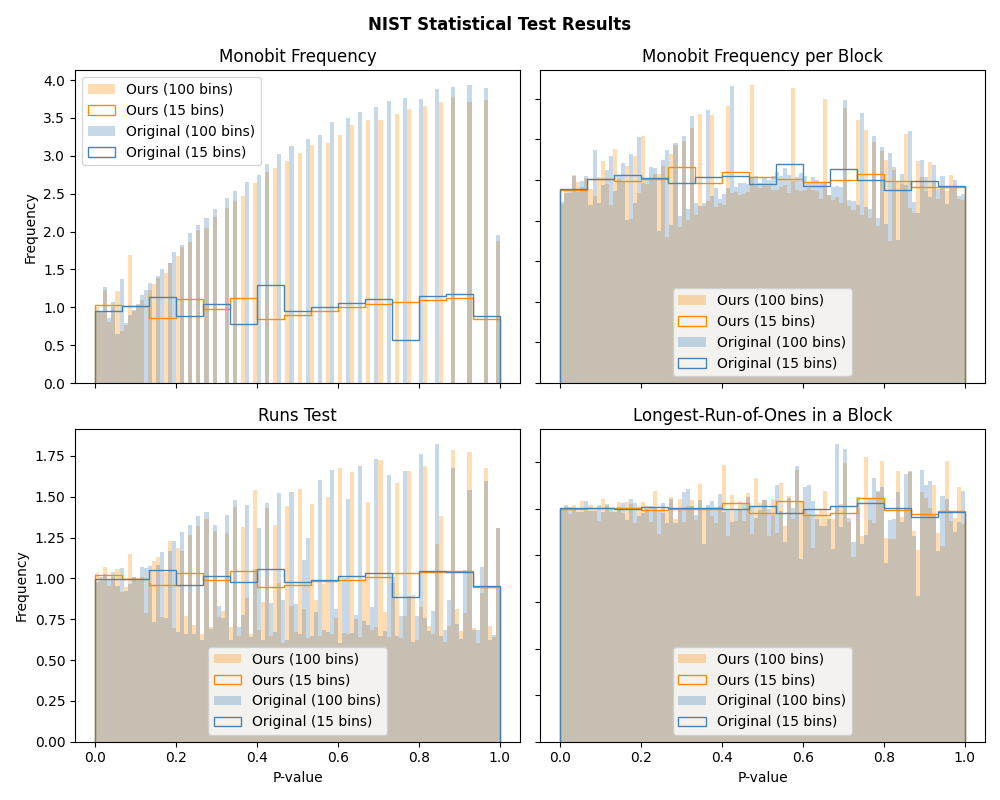
\includegraphics[width=0.9\linewidth]{Images/25-05-19-runwise_comparison_400000h-20n-3m-3p5.png}
    \caption{Distribution of NIST SP 800-22 p-values across 400 000 headers (headerwise evaluation).}
    \label{fig:sp_800-22_hist_headerwise}
\end{figure}
\begin{figure}[H]
    \centering
    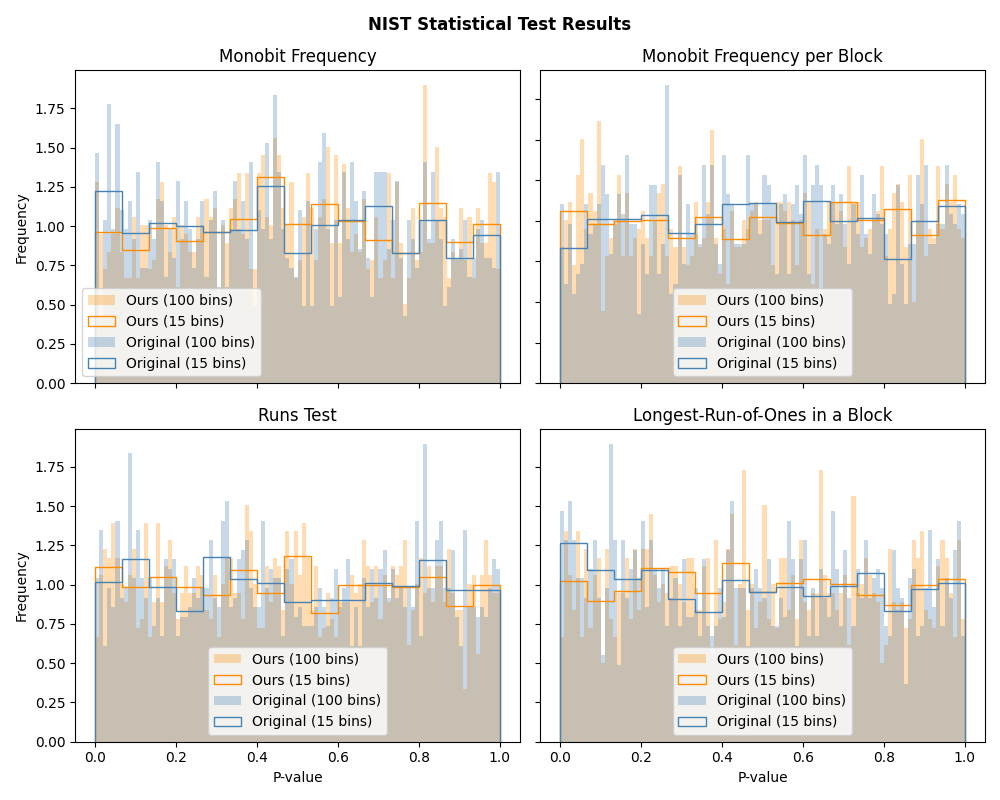
\includegraphics[width=0.9\linewidth]{Images/25-05-19-bitwise_comparison_400000h-20n-3m-3p5.png}
    \caption{Distribution of NIST SP 800-22 p-values per bit across 400 000 headers (bitwise evaluation).}
    \label{fig:sp_800-22_hist_bitwise}
\end{figure}

Some deviations in the histograms arise from the limited size of the bitstrings (1634 or 1792 bits), which introduces quantization effects. 
In particular, the slight distortion in the first test of Figure \ref{fig:sp_800-22_hist_headerwise} reflects the granularity of possible p-values for short inputs. 
Variations in Figure \ref{fig:sp_800-22_hist_bitwise} are due to the small amount of p-values (1634 or 1792).
Increasing the histogram bin size mitigates these artifacts and confirms that the underlying distributions remain approximately uniform.

In both evaluations, the distributions of p-values are approximately uniform, which suggests that headers are statistically indistinguishable from random data, 
and therefore indicates strong linkability resistance, comparable to the original Sphinx implementation.

\subsection{Discussion}

\todo[inline]{Come back to \ref{sec:sp-objectives} objectives and explain
why they hold.}
\section{Conclusion}\label{sec:conclusion}


\bibliographystyle{splncs04}
\bibliography{bib}

\end{document}